\section{Chapter 2 -- Task and Models} % (fold)
\label{sec:task_and_models}
This chapter has two parts, the overall aim of which is to show how a stimulus-response task was used to examine possible category representations of rewards, and then to described how learning in that task was modeled (using a set of reinforcement learning equations).  To that end, and in that order, first the behavioral task is described and its results characterized.  Second, the computational models are rigorously laid out, as are their results.

\subsection{On Task}
\label{sub:to_task}
\subsubsection{What they did, and when}
\label{subsub:whatwhen}
The behavioral task each participant completed consisted of two parts.  Depicted in Figure~\ref{fig:task}. (\emph{top}), the first was a passive learning task wherein participants learned two rewarding perceptual categories by viewing randomly selected black and white sinusoidal gratings.  Each grating (which was on-screen for 2 seconds) was followed by ``Gain \$1'' or ``Lose \$1'' in, respectively, green or red letters (1 second).  The width of the grating's lines and their angles was derived from an information integration (category) distribution (Figure~\ref{fig:II}; borrowed from \citep{Spiering:2008p5008}).  The disappearance of each grating and appearance of the reward was separated by an empty grey screen (1 second).  Each trial terminated in a fixation cross (lasting at least 0.5 seconds). In total then, each trial lasted a total of 4.5 seconds.  The trials for part 1 were spread over an initial training period completed outside the scanner, lasting 126 trials, and an in-scanner refresher lasting 45 trials.  Prior to beginning training participants were, after some preliminaries, instructed to, ``Attend to the screen in order to learn which types of gratings indicate wins and which types indicate losses''.  To minimize any stimulus specific effects, the category parameter distribution (Figure~\ref{fig:II}) to reward (i.e., ``Gain \$1'' or ``Lose \$1'') mapping was randomized for each participant.

Part 2 was a stimulus-response task that replaced classical rewards with an appropriate grating from task 1 (Figure~\ref{fig:task}, \emph{bottom}).  Gratings drawn from the Gain category were used for positive reinforcement, while gratings indicative of losses were used as negative reinforcers.   Each trial began with an abstract black and white ``tree'' stimuli (left most image in bottom of Figure~\ref{fig:task}).  Each ``tree'' deterministically belonged to one of two arbitrary response categories (``q'' or ``w'').  Subjects indicated their response by button press using either the right or left index fingers on a magnet-compatible response box.  The response window lasted up to 2.5 seconds, but ended as soon as a response was made.  Immediately following response the ``tree'' was replaced with a blank grey screen, which was on-screen for half a second and was replaced with a feedback screen.  If the response was correct a \emph{never before experienced} exemplar grating from the gain distribution was used; if the participant was incorrect, a new loss grating appeared instead.  The use of novel gratings forced the subjects to classify each grating prior to inferring its value.  This necessary inference made these rewards incompatible with primary or secondary definitions.  If no response was made, or the wrong button was pressed, the subject's reward was replaced with, ``No response detected'' (these trials were excluded from further analysis).  Feedback always lasted for 1 second and was terminated by a fixation cross (0.5 seconds).  

For the instructions in part 2 participants were told, ``Each tree belongs to either category q or w.  Which is the correct answer though is random.  The shape of trees is meaningless.  To learn the correct response for each tree you must start by guessing.  Use what you learned about the rewarding properties of the gratings from part 1 to learn the right responses.  Remember, a random subset of the Gains and Losses are real.  These mostly determine how much you'll earn for your participation.  So try and earn as much money as possible''.  Instruction for both parts were given orally by the experimenter using a script and Figure~\ref{fig:task} as a visual aid.

Over the course of part 2, participants learned to classify 6 ``trees'', randomly selected at the start of the experiment out of a pool of 22 possible.  Each of the 6 were experienced a total of 28-32 times for a total of 199 trials. The order of the trials in the second half of part 1 and all of part 2 was determined using a genetic algorithm designed to optimize fMRI signal detection, among other considerations.  Most relevant to behavioral analysis, trials were in pseudo-random order with second order counterbalancing.  For remaining details see p\pageref{sub:acquired}.

As part of fMRI data acquisition, 18 participants completed both parts of the task (10 female, mean age of 24, ranging from 21 to 32). Participants were compensated at a base rate of \$15.00 earning up to \$30 more depending on behavioral performance. For the last 30 trials the participant was paid an additional dollar for every correct response and lost a dollar for every incorrect response.  Before beginning experiment participants were told that some trials would count, but were not told until after which trials (i.e., the last 30).  The highest payout was \$45, i.e.,perfect performance, the lowest was 30, indicating near chance behavior for the last 30.  The average payout was \$40.23.

Of the 18 participants, two were removed all analyses as they demonstrated inverse learning (Figure~\ref{fig:sacc}, see \emph{107} and \emph{110}).  Despite reporting a full understanding of the reward contingencies from part 1, in part 2 these participants displayed significant and consistent decreases in performance through time.  Had this learning been in the usual direction it would have been considered better than average performance.  In post task interviews both reported feeling as if they performed above average.  Once they were informed of their inverse performance neither believed it.  It seems possible then that both correctly learned the perceptual characteristics but mis-mapped the value labels, i.e., they got ``Gain'' and ``Loss''  mixed up.  Post-experiment interviews further suggested that both the discarded subjects were under high personal stress.  One subject, who was a PhD student, had his competency exams the next day.  The other completed a 60 mile bike ride an hour prior to participation.  Combined these participant's data suggest that the perceptual and verbal characteristics of the reward categories are independently accessible, and that the verbal label may be more labile than the perceptual distributions.  However given the other participants consistent positive performance and rapid learning it seems these two were a curious but isolated anomaly (Figure~\ref{fig:sacc}).

\begin{figure}[tp]
    \noindent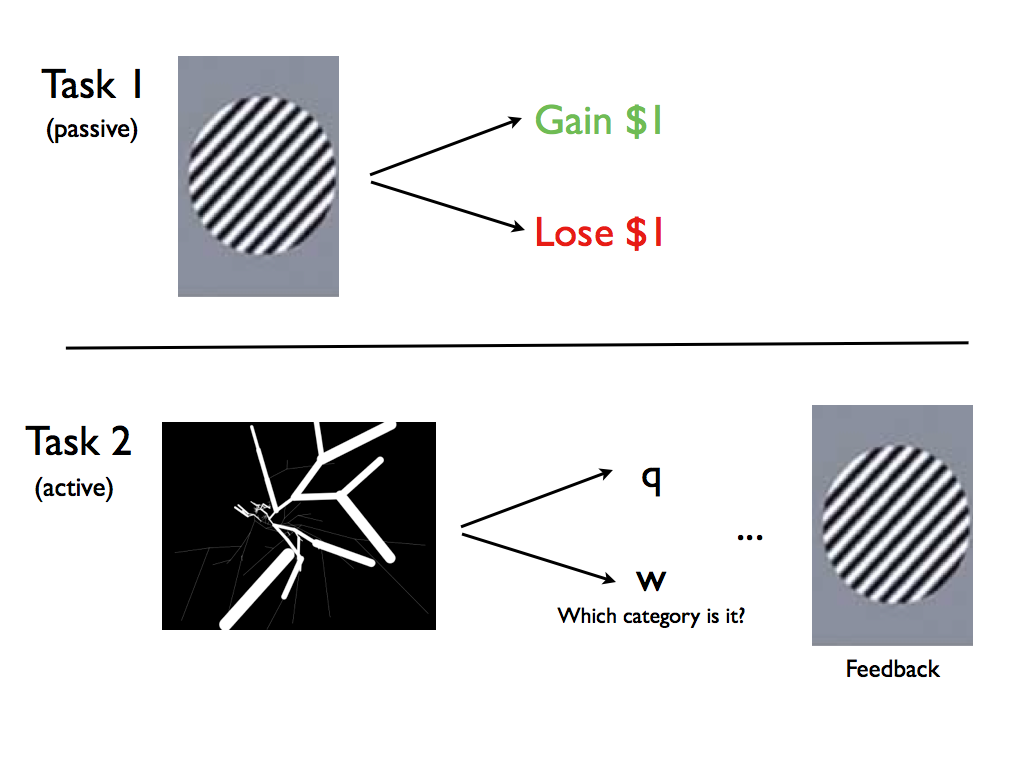
\includegraphics[width=39pc]{f_task}
    \centering
    \caption{Depiction of the behavioral task.  The \emph{top} depicts part 1, the passive learning of the reward categories.  The \emph{bottom} depicts part 2, the stimulus-response learning phase.}
    \label{fig:task}
\end{figure}

\begin{figure}[tp]
    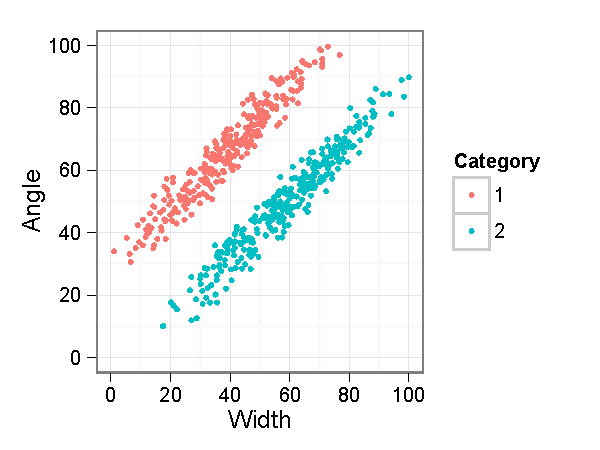
\includegraphics{f_II}
    % TODO -- replace with the good plot; find the good plot again.
    \centering
    \caption{The two sinusoidal grating distributions for the information integration (II) category distributions.   As II categories span the diagonal of the gratings parameter space (line width and angle successful learning requires consideration of both dimensions preventing participants from solving the categorization problem with simple rule-based strategies.}
    \label{fig:II}
\end{figure}

\begin{figure}[tp]
    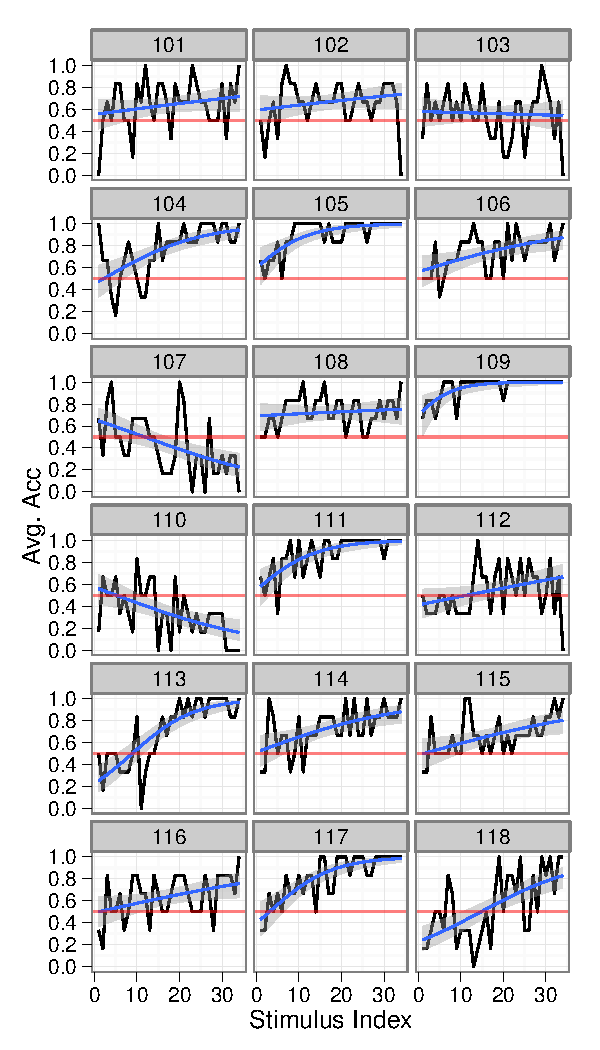
\includegraphics{f_all_sS_acc}
    \centering
    \caption{Average accuracy for each participant (black), averaged for all 6 stimuli by trial (i.e., Stimulus Index), blue line and the grey area represent a binomial regression fit of the data and bootstrapped 95\% confidence intervals, respectively.}
    \label{fig:sacc}
\end{figure}

\begin{figure}[tp]
    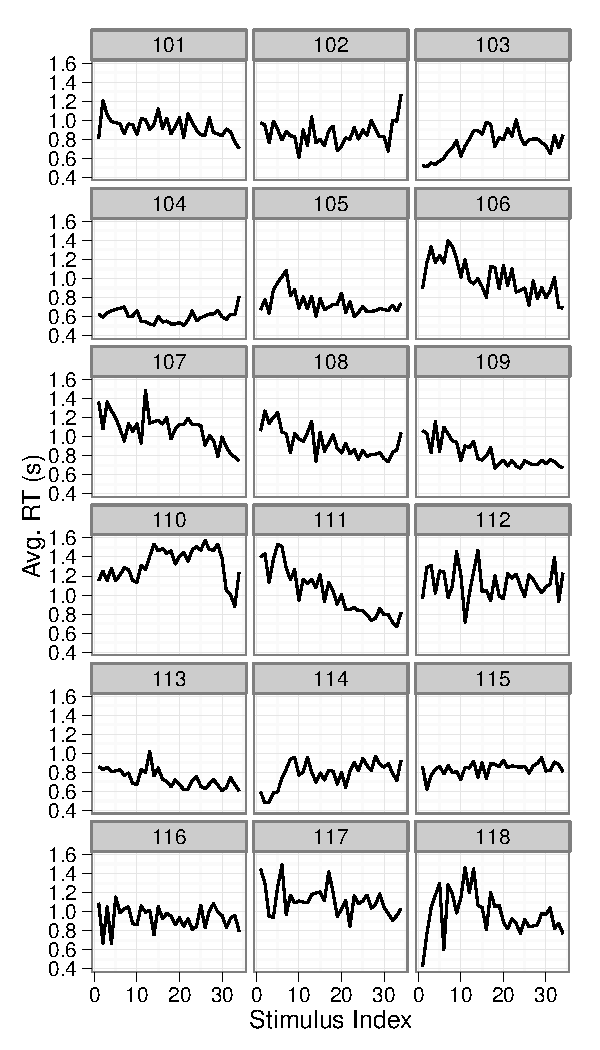
\includegraphics{f_all_sS_rt}
    \centering
    \caption{Mean reaction time for each participant, averaged for all 6 stimuli by trial (i.e., Stimulus Index).}
    \label{fig:srt}
\end{figure}

\subsubsection{Well behaved results}
\label{subsub:wellbehaved}
On an individual basis the lower confidence interval\footnote{All confidence intervals were bootstrapped estimates calculated suing the Hmisc package (\url{http://cran.r-project.org/web/packages/Hmisc/index.html}) in the R programming language (v2.15.1; \url{http://www.r-project.org/})} around the binomial fit of the accuracy data rose to above the chance level (0.5) by the last trial, except for participant 103, who did not learn (Figure~\ref{fig:sacc}).  Many participants (11 of 16) greatly exceeded this minimum criterion, showing above chance learning by trial 10, and nearly all (14 of 16) exceeded chance by trial 20  (Figure~\ref{fig:sacc}).  These individually good performances are reflected in the participants' aggregate performance, which was well above chance by trial 5 (Figure~\ref{fig:meanacc}).  This aggregate learning rate is consistent with past work in the lab using verbal or monetary feedback \citep{Seger:2010p7188,Seger:2005pd}, as it is with other results in other laboratories \citep{ODoherty:2003p6329,Ramnani:2000p6515,Aron:2004p1375,Smith:2008p2803,Poldrack:2008p6839,Ashby:2006p9153,Ashby:2005p4764,Ashby:2005p9152}, indicating that the rewarding categories in present study are behaviorally similar to classical rewards.  The consistency between classical rewards and this task were also reflected in the reaction time measures, which showed a 200 ms decrease over time, bottoming out near 850 (for individual averages see Figure~\ref{fig:srt} and for overall performance see Figure~\ref{fig:meanrt}).  Responses in similar, classically rewarding tasks end with reaction times near 700-800 milliseconds and show similar rates of decline.  The 50-100 ms possible difference in reaction times may be due to the increased difficultly of classifying the rewards compared to simply reading the value of the outcome (e.g., ``Gain \$1'').

\begin{figure}[tp]
    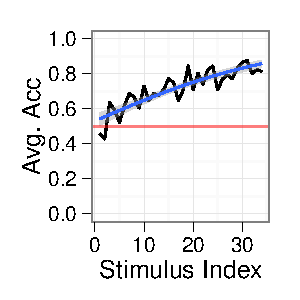
\includegraphics{f_all_mean_acc}
    \centering
    \caption{Mean accuracy (black), averaged over all participants and stimuli, plotted by trial.  The blue line and grey area represent a binomial regression fit of the data and bootstrapped 95\% confidence intervals, respectively.}
    \label{fig:meanacc}
\end{figure}

\begin{figure}[tp]
    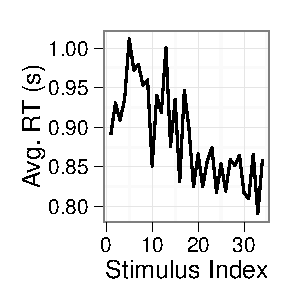
\includegraphics{f_all_mean_rt}
    \centering
    \caption{Mean reaction time (black), averaged over all participants and stimuli, plotted by trial.  The blue line and grey area represent a binomial regression fit of the data and bootstrapped 95\% confidence intervals, respectively.}
    \label{fig:meanrt}
\end{figure}

\subsection{3 Models and 2 Codes}
\label{sub:threemodels}
\subsubsection{Our three models}
\label{subsub:catquant}
Three Rescorla-Wagner-like models were constructed, each using a distinct reward representation.  The first model treated rewards identically to a classical reward (e.g., a 0 for a loss or 1 for a gain).  The second and third devalued each reward based on how similar it was to the category mean.  This similarity metric is (necessarily) simplistic.  As was reviewed on p\pageref{subsub:curves}, there are many proposed models for how the categories are represented.  Likewise, our understanding of the computational implementation of the category learning systems is only just underway \citep{Ashby:2005p9152,Ashby:2006p9153}.  As such there is no obvious way to interlace the hypothesis of rewarding categories with the category learning systems or with the many models of categorization they rely on.  Avoiding such ambiguity, a simpler route driven by Shepard's basic finding \citep{Shepard:1987p9102} was taken.  Whatever the representation and/or category learning system that (may) implement rewarding categories, Shepard's work insists they show an exponential or Gaussian decline with similarity.  For simple stimuli like a light or tone, similarity is measured from the initial training prototype \citep{Guttman:1956p8355}.  However as the task does not have a singular prototype the mean of the parameters for all training trials (i.e., part 1) was used in its place.  This simple substitution makes categories identical to the simplest of the prototype category representations \citep{Rosch:1973p9108,Ashby:1995p9109}, making this a parsimonious yet literature driven first attempt to quantify similarity of rewards.  Therefore, for model two similarity decreased exponentially measured from the training mean, while for model three it decreased following a normal Gaussian (for complete mathematical detail see p\pageref{subsub:codesandfits}).  

\subsubsection{Codes and fits}
\label{subsub:codesandfits}
For each participant and model, the two free parameters ($\alpha$, which controls each model's rate of learning and $\beta$, which controls the steepness of the action selection criterion) were fit using an exhaustive\footnote{With a 0.05 precision, ranging from 0-1 for $\alpha$ and 0-5 for $\beta$} maximum log-likelihood search.  Additionally each model was run using two separate reward coding schemes.  In the first scheme gains were valued as 1 and losses as 0.  The second, which was based on the bivalent monetary value of the rewards, uses 1 and -1 for gains and losses respectively.  The first scheme is universally used in human and animal modeling studies as well as in machine learning, and is the \citep{Sutton:1998p9247} recommended scheme.  However recent recordings of dopaminergic neurons in monkey suggest that the true reward codes are complex, even perhaps redundant \citep{Kim:2006p1063,Matsumoto:2009p7219}.  Among other schemes, they reported firing consistent with a bivalent reward code.  Using the second scheme is merely a first, albeit simple, step in incorporating the potential complexity of dopaminergic firing as observable by the fMRI BOLD signal and in human subjects.

\subsubsection{The incantations}
\label{subsub:incantations}
To restate more formally, a Rescorla-Wagner-like model's value updates were defined by,
\begin{equation} \label{eq:V} V(s_t,a_t) \leftarrow V(s_t,a_t) + \alpha\delta \end{equation} 
\begin{equation} \label{eq:rpe} \delta = r_{(classic,t)} - V(s_t,a_t) \end{equation}
where $\delta$ is the reward prediction error, $s$ is a stimulus, or state (or which there were 6), and $a$ is an action (either ``q'' or ``w'') and $r_{classic}$ (the numerical representation of the rewards) can be coded as either
\begin{equation}
    \label{eq:r1}
    r_{classic}= \{1,0\}
\end{equation}
or 
\begin{equation}
    \label{eq:r2}
    r_{classic}= \{1,-1\}
\end{equation}
but where $r_{classic}(t)$ may also be replaced with
\begin{equation}
    \label{eq:re}
    r_{exp} = r_{classic}S_{exp}
\end{equation}
or
\begin{equation}
    \label{eq:rg}
    r_{gauss} = r_{classic}S_{gauss}
\end{equation}
where $D$ is the Euclidean distance from the width ($w$) and angle ($\theta$) of that trials reward category to the average values from the pre-training ($\bar{\theta}$ and $\bar{W}$; see discussion on part 1 on p\pageref{subsub:whatwhen})
\begin{equation}
    \label{eq:D}\\
    D = \sqrt{(\bar{\theta} - \theta)^2 + (\bar{W}-w)^2}
\end{equation}
is transformed to a Shepard-like similarity metric \citep{Shepard:1987p9102}:
\begin{equation}
    \label{eq:Sexp}\\
    S_{exp} = e^{-D}
\end{equation}
\begin{equation}
    \label{eq:Sgauss}\\
    S_{gauss} = e^{-D^2}
\end{equation}
Consistent with past work, all values are initialized at 0 \citep{Beierholm:2011p8141,BischoffGrethe:2009p4570,Gershman:2009p7207}
\begin{equation} \label{eq:V0} V_{initial} = 0. \end{equation}
and values are transformed to response selection probabilities via the softmax distribution \citep{Sutton:1998p9247,ODoherty:2003p6329}.
\begin{equation}
    \label{eq:softmax}
    p_1(s_t,a_t) = {e^{\beta V_1(s_t,a_t)}\over{e^{\beta V_1(s_t,a_t)} + e^{\beta V_2(s_t,a_t)}}}
\end{equation}
where $V_1$ and $V_2$ are the values for the two response options (i.e., ``q'' and ``w'').
During maximum likelihood parameter selection (p\pageref{subsub:codesandfits}), the $p_1(s_t,a_t)$ values from each trial and some test parameters ($\alpha_{test}$ and $\beta_{test}$) calculate the log-likelihood by,
\begin{equation}
    \label{eq:logL}
    L_{} = \sum{log_e(p_1(s_t,a_t))}
\end{equation}

\subsubsection{Fits and plots}
\label{subsub:fits}
On average none of the three models fit the accuracy data better than the rest (Figure~\ref{fig:logL}).  For brevity's sake each model will be referred to as ``none'', ``exp'' and ``gauss'', corresponding to Eq~\ref{eq:rpe}, Eq.\ref{eq:re}, and Eq.~\ref{eq:rg} respectively.  Nor did the coding scheme impact the fits (``acc'' and ``gl'', matching respectively Eq.~\ref{eq:r1} and Eq.~\ref{eq:r2}; Figure~\ref{fig:logL})).  For ``acc'' the step size parameter (``alpha'' in Figure~\ref{fig:alpha} matching $\alpha$ in Eq.~\ref{eq:V}) increased in ``exp'' compared to the other models.  This increase was expected as the exponential similarity metric can sharply decrease the magnitude of each value update, requiring an increase in $\alpha$ to compensate.  A similar trend was observed for the temperature parameter (``beta'' in Figure~\ref{fig:beta}, matching $\beta$ in Eq.~\ref{eq:softmax}). The more equiprobable each action is the larger the temperature parameter.  As such the increase for ``exp'' means participant's choices are more likely to change from trial to trial, which is again consistent with a decrease in update magnitudes.

Importantly the intra-subject variability in $\alpha$ and $\beta$ was low, as demonstrated by the small standard error of both parameters (Figure~\ref{fig:alpha} and~\ref{fig:beta}).  Consistent parameter estimates between subjects support the use of subject-level parameters in the fMRI analyses, which in other hands have been reported to be too noisy to be reliable \citep{Daw:2011p7995,Seymour:2007p7585,ODoherty:2003p6329}.  Using subject-level parameters is a crucial step in assessing and maximizing model quality. The goal of any model of human behavior is to make good predictions for individual cases not just for aggregates of tens or hundreds of participants \citep{Daw:2007p9346}.  However aggregates prediction is the norm in reinforcement learning models of human behavior (for examples see, \citep{Daw:2011p7995,Seymour:2007p7585,ODoherty:2003p6329}).

\begin{figure}[tp]
    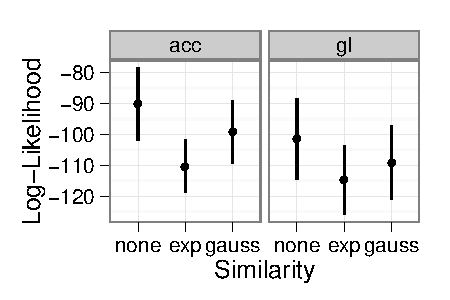
\includegraphics{f_logL}
    \centering
    \caption{Average negative log-likelihoods for each of the models and coding schemes.  Error bars represent standard errors.}
    \label{fig:logL}
\end{figure}

\begin{figure}[tp]
    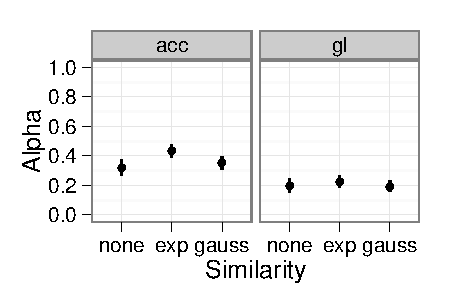
\includegraphics{f_alpha}
    \centering      
    \caption{Average alpha values for each of the models and coding schemes.  Error bars represent standard errors.}
    \label{fig:alpha}
\end{figure}

\begin{figure}[tp]
    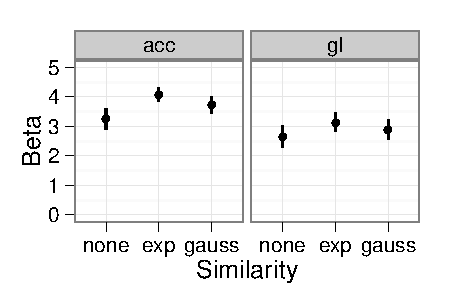
\includegraphics{f_beta}
    \centering
    \caption{Average beta values for each of the models and coding schemes.  Error bars represent standard errors.}
    \label{fig:beta}
\end{figure}

The fit reinforcement learning models for every participant and coding scheme can be found in Figure~\ref{fig:rpeacc} -~\ref{fig:valuegl}.  In the traditional formulation, where similarity does not impact reward value (e.g., see Figure~\ref{fig:rpeacc} or~\ref{fig:rpegl}) the reward prediction error decreases with learning, eventually plateauing at 0, for strong examples see subjects \emph{102}, \emph{105} and \emph{111} in the ``none'' column of Figure~\ref{fig:rpeacc}.  In contrast, both similarity models, ``exp'' and ``gauss'', never fully plateaued (again see Figure~\ref{fig:rpeacc}).  In the context of the models, this is expected.  Each grating will, in all likelihood, be non-identical to the mean. However as the parameter mean is the asymptotic expectation, reward prediction errors happen even after learning is complete.  In the big picture, this is the desired behavior.  The similarity adjusted models are trying to capture the case where a reward's value may vary in ways that are not predictable \emph{a priori}; Given the massive multiplicity of possible outcomes in the world it is unlikely to find the same one multiple times.  Small prediction error should then continue without end, as happens in these models.

When comparing ``exp'' and ``gauss'' models, you'll see the former appears to have lower magnitudes (Figure~\ref{fig:rpeacc}).  Examining density plots composed of all participants data confirms this observation (Figure~\ref{fig:denrpe}).  The density plot also reveals that ``exp'' prediction errors are diminished more rapidly than their ``gauss'' counterparts (a pattern most clearly scene in the left panel of Figure~\ref{fig:denrpe}).  

Regardless of model class, between the two reward codes there are substantial differences in reward prediction behavior.  The $\{1,-1\}$ (denoted in these plots as ``gl'') scheme leds to substantially more negative deflections that the $\{1,0\}$ scheme (``acc'') (compare Figure~\ref{fig:rpegl} and ~\ref{fig:rpeacc} as well as the \emph{left} and \emph{right} panels of~\ref{fig:denrpe}).   

Value estimates for the two similarity adjusted rewards (i.e., ``exp'' and ``gauss'') were generally less than the alternative classic model (``none'' in Figure~\ref{fig:valueacc} and~\ref{fig:valuegl}).  However, as a consequence of their reduced dynamic range, the similarity adjusted model's value terms grew more rapidly, for example examine participants \emph{105} and \emph{109} in Figure~\ref{fig:valueacc}.  In these cases both the similarity value terms approached their maximum by trial 50 whereas ``none'' (the unadjusted term) took until trial 150.  That is, taking into account the uncertainty of each reward's worth led to an increase in the learning rate.  This increase was independent of the reward coding scheme (i.e., see also Figure~\ref{fig:valueacc}-~\ref{fig:valuegl}).  

The coding scheme's impact on the value terms was two fold.  First, as losses led to larger prediction errors using the ``gl'' scheme (-1 compared to 0), value increased faster for ``acc'' (see Figure~\ref{fig:valueacc} and~\ref{fig:valuegl} as well as~\ref{fig:denvalue}).  Second, and most strikingly, ``gl'' led to negative value estimates of the undesirable choices (Figure~\ref{fig:valuegl} compared to~\ref{fig:valueacc}).  While, so far as I'm aware, no reinforcement learning model of human or animal have considered negative value estimates, there is empirical support.  As reviewed on p\pageref{subsub:fclt}, orbital frontal and ventral medial frontal cortices encode the absolute value of rewarding or punishing outcomes \citep{ODoherty:2001p2423,Hornak:2004p6234}.  As such, neural correlates of reinforcement learning derived negative value estimates might serve as an important link between theoretical and empirical findings on economic valuation.  It might also serve as a link between reinforcement learning and affective/motivational processing \citep{Knutson:2005p1627,Delgado:2004p6665}.

\begin{figure}[tp]
    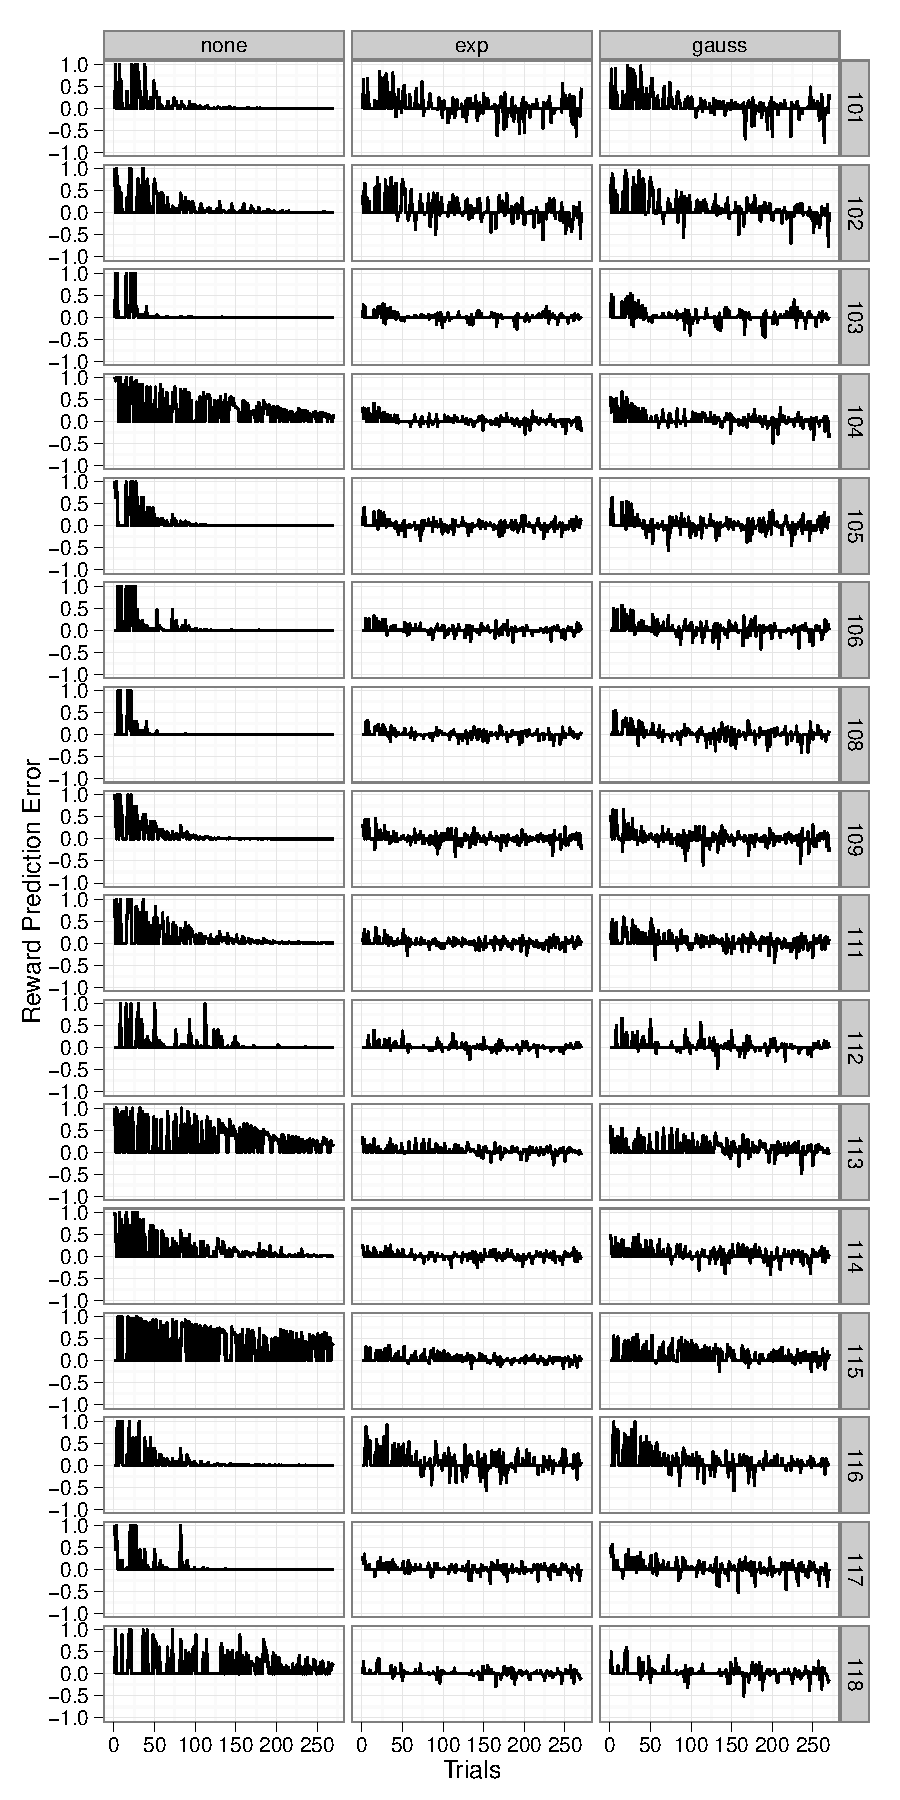
\includegraphics[width=0.6\textwidth]{f_rpe_acc}
    \centering
    \caption{Reward prediction errors for each of the three models plotted for each trial in the experiment, based on the $\{1,0\}$ coding scheme, which also represents the min-max range of the y-axis.  Each row is a single subject's data.  Each column matches one of the three models, classified by their similarity metric.}
    \label{fig:rpeacc}
\end{figure}
\begin{figure}[tp]
    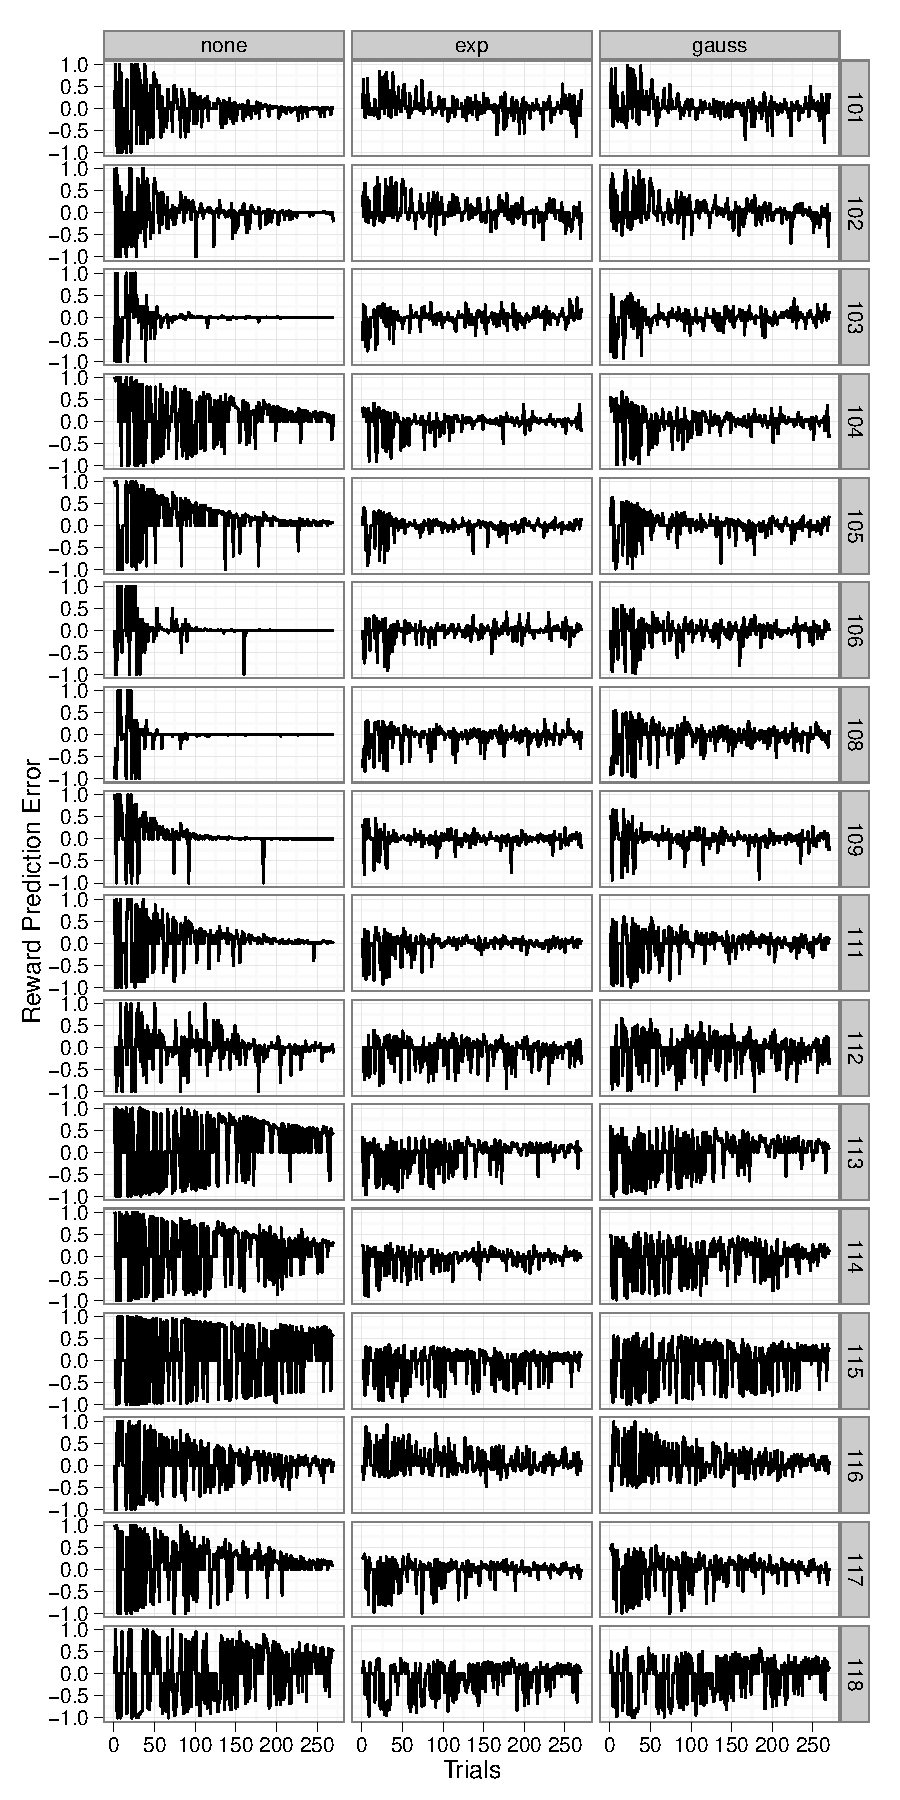
\includegraphics[width=0.6\textwidth]{f_rpe_gl}
    \centering
    \caption{Reward prediction errors for each of the three models plotted for each trial in the experiment, based on the $\{1,-1\}$ coding scheme, which also represents the min-max range of the y-axis.   Each row is a single subject's data.  Each column matches one of the three models, classified by their similarity metric.}
    \label{fig:rpegl}
\end{figure}

\begin{figure}[tp]
    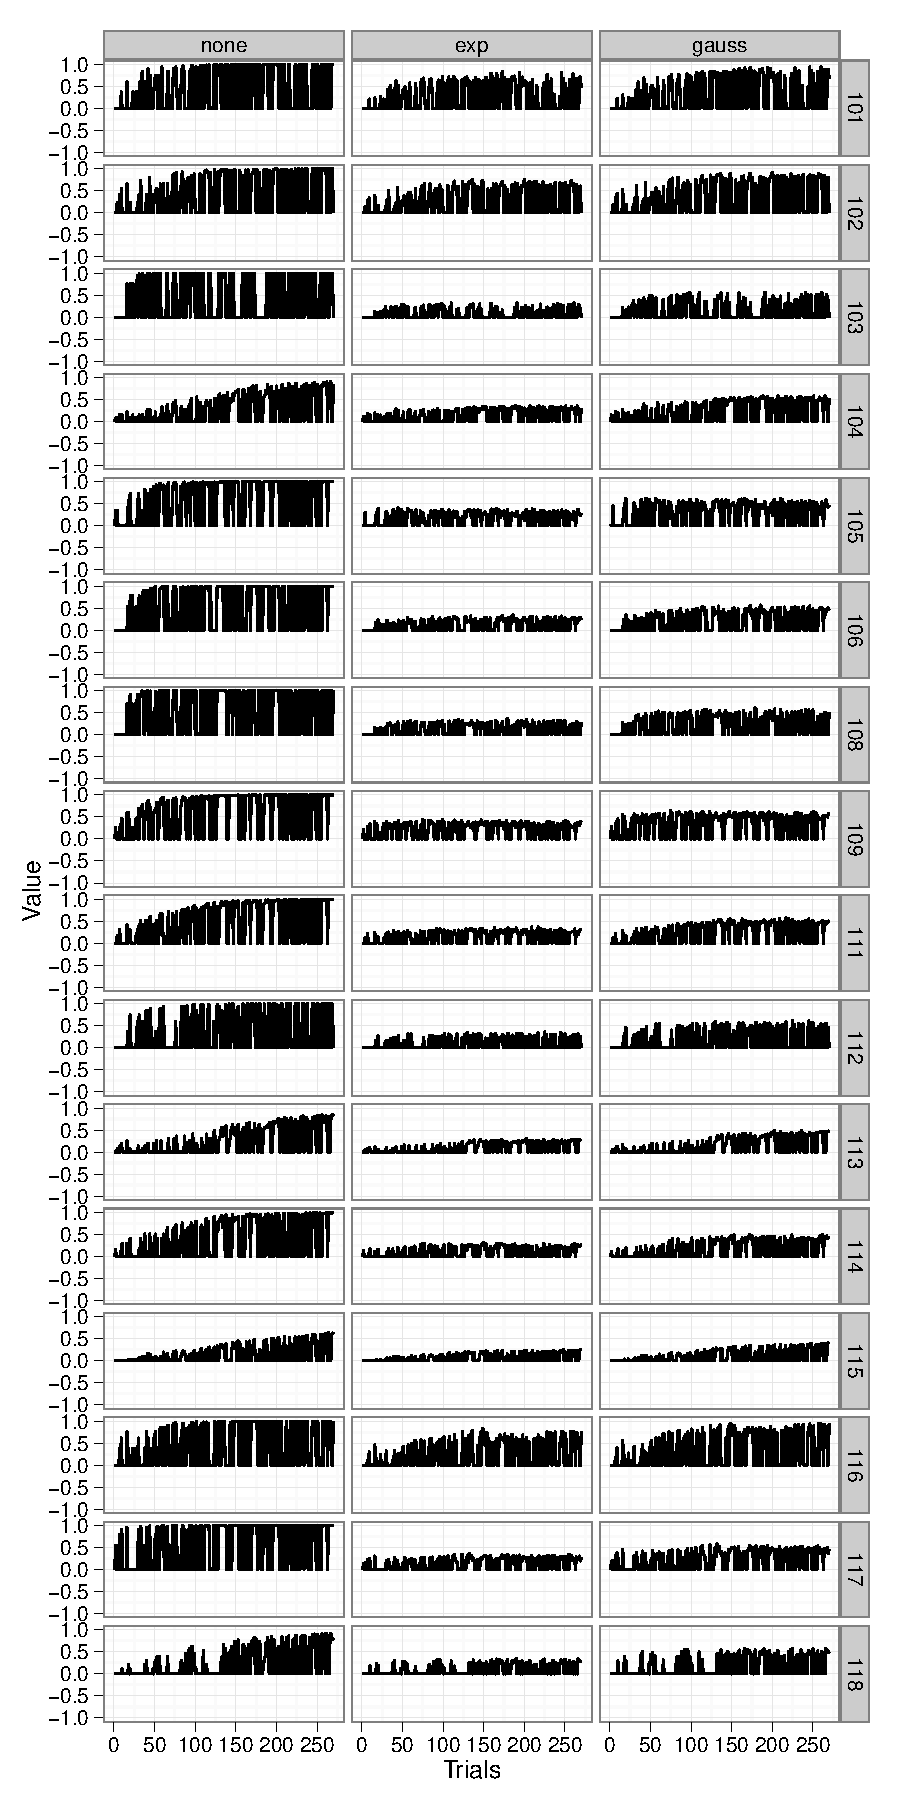
\includegraphics[width=0.6\textwidth]{f_value_acc}
    \centering    
    \caption{Value estimates for each of the three models plotted for each trial in the experiment, based on the $\{1,0\}$ coding scheme, which also represents the min-max range of the y-axis.  Each row is a single subject's data.  Each column matches one of the three models, classified by their similarity metric.}
    \label{fig:valueacc}
\end{figure}
\begin{figure}[tp]
    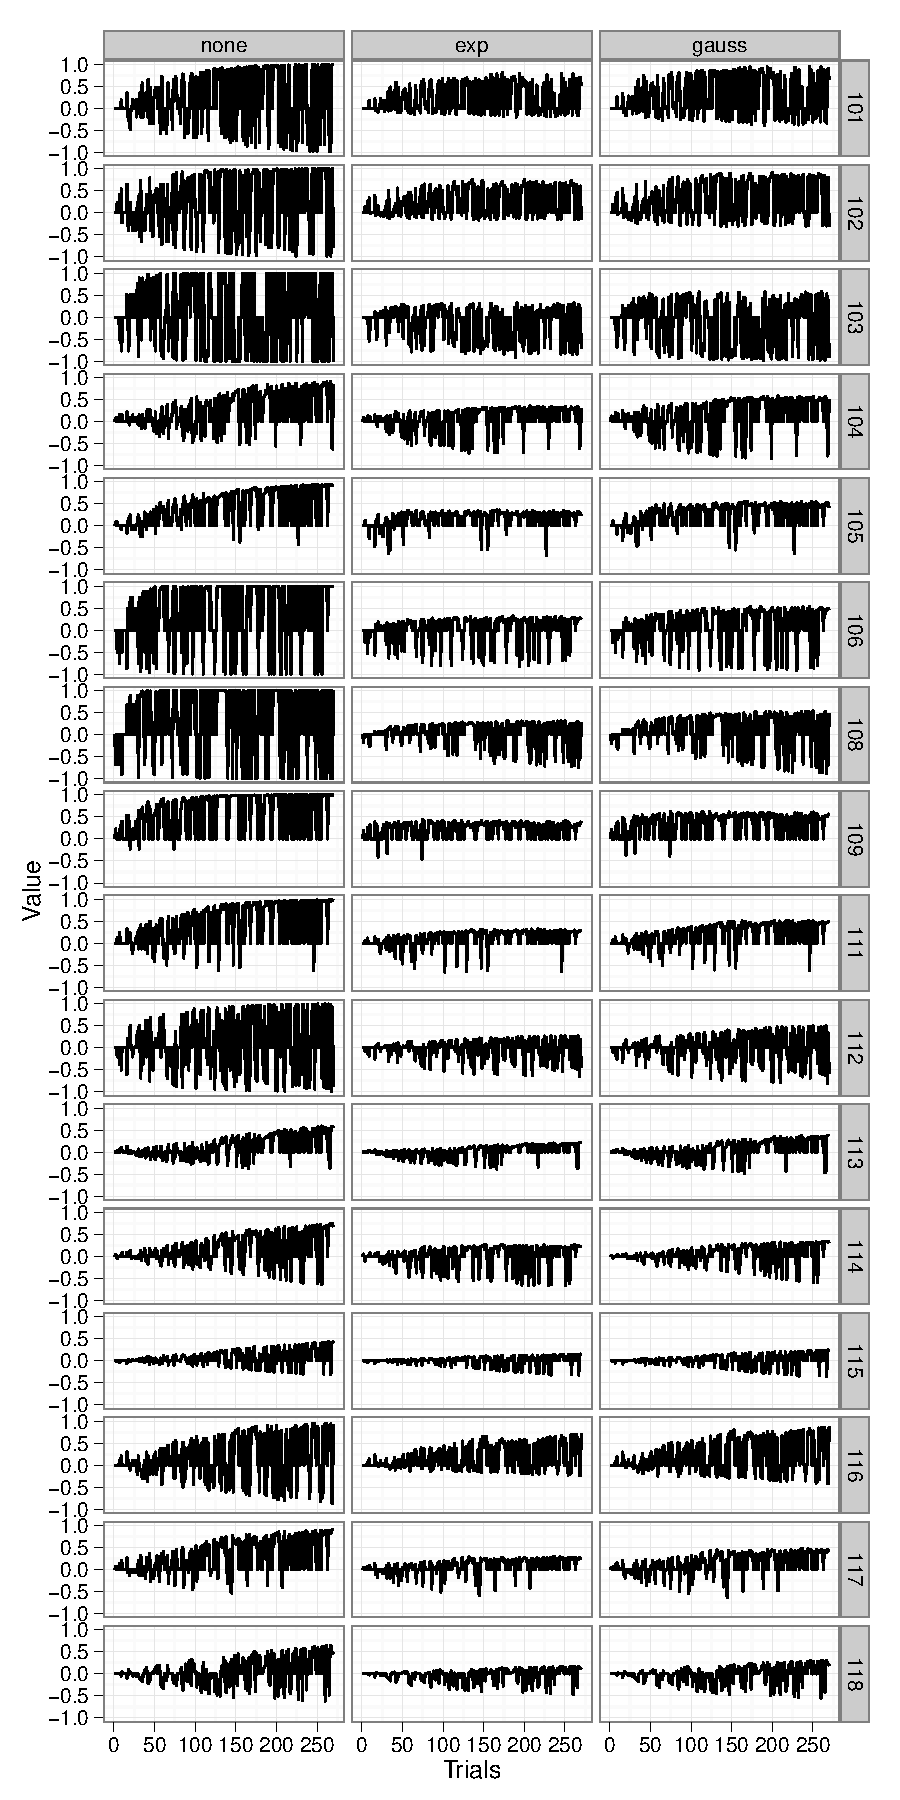
\includegraphics[width=0.6\textwidth]{f_value_gl}
    \centering
    \caption{Value estimates for each of the three models plotted for each trial in the experiment, based on the $\{1,-1\}$ coding scheme, which also represents the min-max range of the y-axis.   Each row is a single subject's data.  Each column matches one of the three models, classified by their similarity metric.}
    \label{fig:valuegl}
\end{figure}
\begin{figure}[tp]
    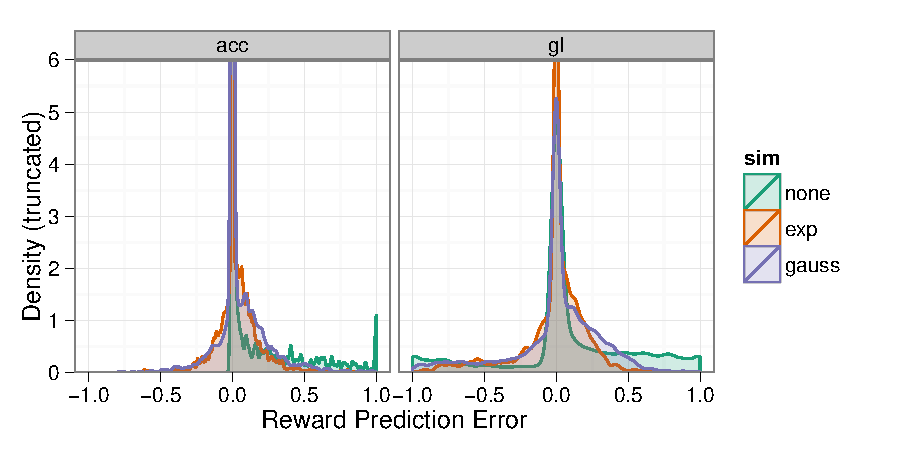
\includegraphics{f_density_rpe}
    \centering
    \caption{Density of reward prediction errors for all subjects.  The y axis is truncated at 6 to allow clear visualization of non-zero values.}
    \label{fig:denrpe}
\end{figure}

\begin{figure}[tp]
    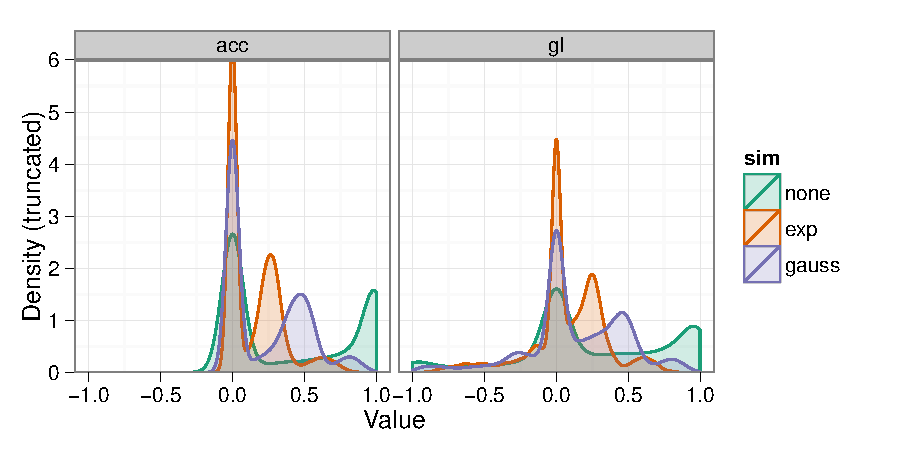
\includegraphics{f_density_value}
    \centering
    \caption{Density of value estimates for all subjects.  The y axis is truncated at 6 to allow clear visualization of non-zero values.}
    \label{fig:denvalue}
\end{figure}
\clearpage